\chapter{The Standard Model of particle physics}
\chaptermark{The Standard Model of particle physics}  
\thispagestyle{plain}  % First page has default style
\pagestyle{chapterpages}
The \ac{SM} of particle physics~\cite{Glashow_StandardModel_1,Weinberg_StandardModel_1,StandardModel_3,Standard_Model4,StandardModel_3} is our current best theoretical framework underpinning our understanding of the subatomic world, providing a description of fundamental elementary particles and their interactions via the electromagnetic force, weak nuclear force and the strong nuclear force. The fourth fundamental force of nature, Gravity, is absent from the SM, highlighting one of its key limitations. However, in high-energy physics experiments, where the interactions of subatomic particles are being studied, the omission of gravity is considered a safe simplification. Extremely powerful predictions have emerged from this theoretical framework, with its greatest accomplishments being the prediction~\cite{Higgs_1} and subsequent discovery of the Higgs boson in 2012~\cite{Higgs_ATLAS,Higgs_CMS}. Despite its success, the Standard Model has its limitations. Along with the absence of gravity, it leaves several fundamental questions unanswered, such as the nature of neutrino oscillations~\cite{Neutrino_Oscillations}, the existence of dark matter~\cite{DarkMatter}, the hierarchy problem~\cite{HierarchyProblem}, and the matter-antimatter asymmetry in the universe~\cite{MatterAntimatter}, which cannot be fully explained by the predicted amount of CP violation, driving the field to look for explanations beyond the SM. In the pursue of \ac{BSM} physics, a deep understanding of the SM theory is crucial. This is the goal of this chapter aiming to establish the base foundation for this work, the SM, by exploring the fundamental blocks of the theory, including its particle content, interactions, and the Higgs mechanism.

\section{Particle content and fundamental interactions}

Built upon the theoretical framework of \ac{QFT}~\cite{QFT}, the SM is a renormalisable theory, where the physical particles observed in nature emerge as quantised excitations of underlying relativistic fields with the interactions between them, themselves being desribed by the exchange of particles. These two groups of particles constitute the particle content of the SM, as shown in Fig.~\ref{Figure:Introduction_1}.

\begin{figure}[h]
\centering
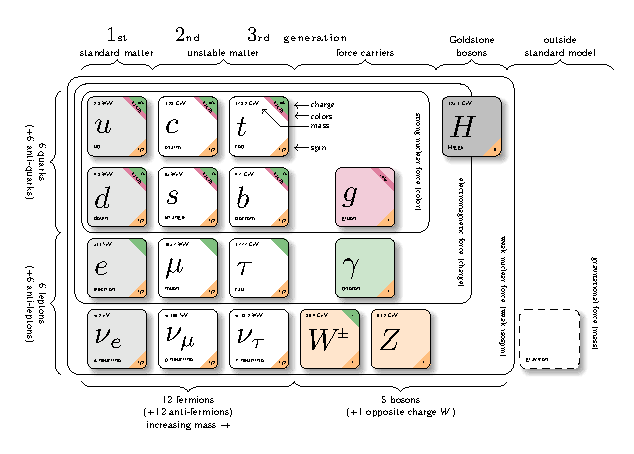
\includegraphics[width= 1\textwidth]{Figures/Introduction/Particles.pdf}
\caption{Diagram of the particle content of the SM. For each fundamental particle, the charges, colour and spin quantum numbers are available. The measured masses for all fermions and gauge bosons are taken from Ref.~\cite{ParticleMasses} with the exception of the Higgs mass which is taken from Ref.~\cite{Higgs_Mass}.}
\label{Figure:Introduction_1}
\end{figure}

The elementary particles of the SM are fundamental objects which are neither bound states of other particles nor composite. These fundamental constituents of matter, known as fermions, are particles with half-integer spin, and are further split into two types: quarks, that can interact via the strong force and leptons which cannot.  The electron, the electron-neutrino, the up-quark and the down-quark comprise the first generation of fermions in the SM, whilst the second and third generations of fermions are heavier replicas \ie same charge but, different masses. Each SM fermion has a corresponding antiparticle with the same mass but opposite quantum numbers: parity and charge.

The interactions of these matter particles are mediated by the exchange of particles with integer-spin, the gauge bosons. All fermions interact via the weak force, mediated by the exchange of massive vector bosons, the $\text{W}^\pm$ and the Z bosons. The electrically neutral leptons, neutrinos, do not interact with the massless photon field, $\gamma$, excluding them from the electromagnetic interaction. Only quarks, on the other hand, possess colour charge, coming in three possible states: red, green and blue, allowing them to participate in strong interactions mediated by the exchange of the massless gluon (g). 

\section{Foundation of the fundamental interactions}

In the core of QFT and the SM lies the principle of symmetry, with the Lagrangian density serving as the starting point of describing fundamental interactions. Fundamental laws are closely tied to symmetries, as demonstrated by N\"{o}ether's theorem: a conservation law is implied by the invariance of a Lagrangian under a continuous transformation (symmetry). A striking example of the deep connection between fundamental interactions and symmetry principles is the conversation of angular momentum, defined by a Lagrangian which is invariant under rotational transformations. Built on the principle of local gauge invariance is the SM Lagrangian. Imposing this invariance gives rise to gauge boson fields, whose interactions with the fundamental matter fields are governed by the symmetry group of the gauge transformation. The gauge symmetry group of the SM is

\begin{equation}
G_{SM} = SU(3)_{C} \otimes SU(2)_{L} \otimes U(1)_{Y}
\end{equation}

\subsection{Quantum Chromodynamics}

\ac{QCD} is the theory that describes strong interactions, governed by the $SU(3)_{C}$ gauge symmetry, with colour charge as the associated quantum number. The mediators of the QCD are the eight massless gluons corresponding to the eight generators of the SU(3) local gauge symmetry. An interesting property of the strong force mediators is that themselves they carry colour charge, allowing them to interact with quarks but, also with themselves. This gluon self-interaction property modifies the strength of the interaction ($\alpha_{S}$) causing it to decrease as a function of the interaction energy scale, hence why $\alpha_{S}$ is referred to as a running coupling constant.

An important consequence of this, is the QCD phenomenon referred to as asymptotic freedom~\cite{AsymptoticFreedom_1,AsymptoticFreedom_2}, where at very high energies (short distances), such as the deep scattering energies at the LHC, $\alpha_{S}$ decreases approaching zero, signifying that the interactions between quarks and gluons are very weak. In this scenario, quarks and gluons behave as quasi-free particles inside the protons and neutrons, described well by perturbation theory. On the contrary, the  low energy regime of QCD is non-perturbative because of the coupling constant becoming increasingly large. In this regime, partons (quarks and gluons) are observed in composite, colourless states known as hadrons. This phenomenon is known as colour confinement and is responsible for the absence of isolated colour-charged particles in nature. 

As a consequence of colour confinement, in high-energy collisions, high-energy quarks and gluons are observed as jets~\cite{Hadronisation_Jets} of colourless particles formed through a process known as hadronisation. In the context proton-proton (pp) collisions, highly energetic partons fly away from the interaction point. As the partons separate, the colour field between them partons can be thought as if it is being squeezed in a tube, with the energy in the field becoming increasingly larger with distance. Once that energy becomes sufficient a new quark-antiquark pair is produced, separating the colour field into smaller segments. Eventually the formation of colourless hadrons occurs when the quark-antiquark pairs have sufficiently low energy. This resulting cascade of collimated hadrons forms what is observed as a jet.

\subsection{Electroweak theory}

In the 1960s, Glashow~\cite{Glashow}, Salam~\cite{Salam} and Weinberg~\cite{Weinberg} discovered independently that a unified picture of the electromagnetic and weak interactions could be constructed. Their proposal was to develop the electroweak theory incorporating the characteristics of both interactions by associating them with the $SU(2)_{L}$ $\otimes$ $U(1)_{Y}$ symmetry group. Specifically, the electroweak Lagrangian is required to be invariant under local transformations of this symmetry group.

The generators, $T_{i}$, of the non-Abelian $SU(2)_{L}$ symmetry group are the 3 Pauli-spin matrices with weak isospin, $I$, being the associated conserved quantity. On the other hand, the Abelian $U(1)_{Y}$ symmetry has a single generator and operates on the weak hypercharge, $Y = 2(Q-I_{3})$, which is related to the electromagnetic charge $Q$ and the third component of the weak isospin, $I_{3}$. Imposing gauge invariance under this symmetry group, four gauge fields emerge: three weak isospin fields, $W_{\mu}^{(i)}$ (i=1,2,3), and the weak hypercharge field, $B_{\mu}$. These gauge fields can be rotated in the physical fields for the photon, the W and the Z bosons, as follows:

\begin{equation}
\begin{array}{c}
A_{\mu} = + B_{\mu} \cos{\theta_{W}} + W_{\mu}^{(3)} \sin{\theta_{W}}, \\
Z_{\mu} = - B_{\mu} \sin{\theta_{W}} + W_{\mu}^{(3)} \cos{\theta_{W}}, \\
W_{\mu}^{\pm} = \frac{1}{\sqrt{2}} (W_{\mu}^{(1)} \mp iW_{\mu}^{(2)}),
\end{array}
\label{Equation:Introduction_PhysicalGaugeFields}
\end{equation}

where $\theta_{W}$ is the weak mixing angle that is related to the weak and electromagnetic coupling constants shown by $g$ and $g'$ respectively, $\theta_{W} = \arctan(g'/g)$.

A key feature of $SU(2)_L$ is that only couples to left-handed fermion fields, indicated by the subscript "L". This is an experimentally verified result, emerging from parity being violated in the weak interaction~\cite{ParityViolation}. Using chiral operators, $P_{L/R}$, the fermion spinor fields ($u$) can be decomposed into left-handed ($u_{L}$) and right-handed ($u_{R}$) chiral components. Under the EW symmetry group, the left-handed components transform as doublet whereas the right-handed components are placed into weak-isospin singlets remaining unaffected by the $SU(2)$ local gauge transformation~\cite{Parity_LHanded}.

Despite, beautifully unifying the electromagnetic and weak interactions into a single theory, a fundamental issue persists because of non-zero mass measurements of the W and Z bosons~\cite{W_Z_MassMeasurements_1,W_Z_MassMeasurements_2}. This is clearly omitted from the EW Lagrangian as the inclusion of the required terms would break the underlying gauge symmetry. Mass terms of the form ${m_{W}^2 W_{\mu}^{-} W^{+\mu}}$ and $\frac{1}{2} m_{Z}^{2} Z_{\mu} Z^{\mu}$ are not invariant under the $SU(2)_{L}$ $\otimes$ $U(1)_{Y}$ symmetry group. This extends also to fermions with mass terms of the form, $m\overline{\psi}\psi = m(\overline{\psi}_{R}\psi_{L} + \overline{\psi}_{L}\psi_{R})$ as the inclusion of such a term in the EW Lagrangian would break the symmetry because of left-handed and right-handed chiral components transforming differently. The answer to this puzzle came through the Higgs mechanism, which is discussed in Section~\ref{Section:Introduction_HiggsMechanism}.

\section{Higgs mechanism}
\label{Section:Introduction_HiggsMechanism}
First proposed back in the 1960s by Englert and Brout~\cite{Englert_Brout}, Higgs~\cite{Higgs_2}, and Guralnik, Hagen and Kibble~\cite{Guralnik_Hagen_Kibble,Kibble_1}, the Higgs mechanism provides a way to generate mass while preserving the local gauge invariance of the SM. It is based on the principle of \ac{SSB} where, the Lagrangian of a system remains invariant under a certain symmetry group, but the vacuum of state of the system does not~\cite{SSB_Definition}. 

In the context of EW theory, the symmetry is broken by introducing a gauge invariant complex scalar $SU(2)_{L}$ doublet, $\phi$. The doublet acquiring a non-zero \ac{VEV} spontaneously breaks the symmetry reducing the EW symmetry group to $U(1)_{EM}$.

\[
\phi =
\begin{pmatrix}
\phi^{+} \\
\phi^{0} 
\end{pmatrix}
= \frac{1}{\sqrt{2}} \begin{pmatrix}
    \phi_{1} + i\phi_{2} \\
    \phi_{3} + i\phi_{4}
\end{pmatrix}
\]

This doublet, known as the Higgs field, contributes four \ac{dof} to the SM Lagrangian; one for the real part and one for the imaginary part of each component. The corresponding Lagrangian for the Higgs field is

\begin{equation}
    \mathcal{L}_{\text{Higgs}} = (D_{\mu} \phi)^{\dagger}(D^{\mu}\phi) - \underbrace{(\mu^{2}\phi^{\dagger}\phi + \lambda(\phi^{\dagger}\phi)^2)}_{\text{V($\phi$)}}
\label{Equation:Introduction_HiggsLagrangian}
\end{equation}

where $D_{\mu}$ is the covariant derivative,

\begin{equation}
    D_{\mu} = \partial_{\mu} + i\frac{g}{2}\vec{T}\cdot\vec{W_{\mu}} + i\frac{g'}{2}YB_{\mu}
\end{equation}

The second term in Eq.~\ref{Equation:Introduction_HiggsLagrangian} is the Higgs potential, which depends on the Higgs field and two real parameters, $\mu^{2}$ and $\lambda$. The vacuum state of the Higgs field corresponds to the minimum of this potential, imposing constraints on the parameters: $\lambda$ must be positive ($\lambda > 0$) to ensure a finite minimum, and $\mu^{2}$ must be negative ($\mu^{2} < 0$) to allow for a non-zero VEV. These constraints result in a potential with an infinite set of degenerate minima, where the Higgs field satisfies,

\begin{equation}
    \phi^{\dagger}\phi = -\frac{\mu^{2}}{2\lambda} = \frac{\nu^2}{2}
\end{equation}

The goal of SSB in the Higgs mechanism is to generate masses for the three massive gauge bosons and the fundamental particles.  Noticeably, the neutral photon still needs to remain massless because of the $U(1)_{EM}$ symmetry being preserved after the symmetry breaking. To satisfy this, the minimum of the Higgs potential must correspond to a non-zero VEV only for the neutral scalar field $\phi^{0}$~\cite{Higgs_VacuumState_Choice},

\begin{equation}
    <0|\phi|0> = \frac{1}{\sqrt{2}} \begin{pmatrix}
        0 \\
        \nu
    \end{pmatrix}
\end{equation}
 
Before expanding the Higgs field around its minimum to study the consequences of SSB, it is important to recall Goldstone's theorem~\cite{Goldstone}, predicting the emergence of a massless scalar (Goldstone) boson after the spontaneous breaking of a continuous symmetry. Out of the four dof introduced by the Higgs field, the three associated with the broken symmetry generators become Goldstone bosons, appearing as massless scalar fields in the Lagrangian. Gauge invariance guarantees that the choice of gauge does not affect the physical predictions of the theory, allowing us to eliminate the Goldstone bosons from the Lagrangian by making an appropriate local gauge transformation. This is referred to as the unitary gauge where the dof associated with the massless Goldstone bosons are replaced with new degrees of freedom corresponding to the longitudinal polarisation states of the gauge bosons ($W^{\pm}/Z$). In the unitary gauge, the Higgs field can be re-expressed as,

\begin{equation}
    \phi = \frac{1}{\sqrt{2}}\begin{pmatrix}
        0 \\
        \nu + h
    \end{pmatrix} 
    \label{Equation:Introduction_HiggsField_2}
\end{equation}

where h is the physical Higgs field, the fourth dof in the Higgs sector.

The term in the Lagrangian responsible for generation of the masses of gauge bosons is $(D_\mu\phi)^\dagger(D^\mu\phi)$. Substituting Eq.~\ref{Equation:Introduction_HiggsField_2} into this term and expressing the $B_\mu$ and $W_{\mu}^{(i)}$ fields in terms of physical $Z_\mu$ and $W_{\mu}^{\pm}$ states using Eq.~\ref{Equation:Introduction_PhysicalGaugeFields}, we obtain the following weak boson mass terms,

\begin{equation}
    \mathcal{L}_{\text{Higgs}} \supset \frac{1}{4} g^2 \nu^2 W^{+\mu}W_{\mu}^- + \frac{(g^2+g'^2)\nu^2}{8} Z_\mu Z^\mu
\label{Equation:Introduction_HiggsLagrangian_2}
\end{equation}

Using the known form of a mass term for a spin-1 gauge boson, the masses of the $W^\pm$ and the Z bosons can be expressed in terms of the $SU(2)_{L}$ $\otimes$ $U(1)_{Y}$ gauge couplings and the Higgs VEV ($\nu = 246 \GeV$) as,

\begin{equation}
\begin{array}{c}
    m_W = \frac{1}{2}g\nu \\
    m_Z = \frac{1}{2}\nu\sqrt{g^2+g'^2}
\end{array}
\end{equation}

Importantly in this physical basis, the neutral gauge boson associated with the $\text{A}_\mu$ field remains massless while the physical Higgs field also appears in the Lagrangian with the associated terms being,

\begin{equation}
    \mathcal{L}_{\text{Higgs}} \supset \underbrace{\frac{1}{2} \partial_\mu h \, \partial^\mu h - \lambda \nu^2 h^2}_{\text{massive scalar boson } h}
    \underbrace{- \lambda \nu h^3 - \frac{1}{4} \lambda h^4}_{\text{Higgs self-interactions}}
\label{Equation:Introduction_HiggsLagrangian_3}
\end{equation}

According to Eq.~\ref{Equation:Introduction_HiggsLagrangian_3}, the mass of the scalar boson field in given by $\text{m}_H = \sqrt{2\lambda}\nu$. This Lagrangian also contains terms describing the trilinear and quartic self-interactions of the Higgs boson for which the relevant Feynman diagram are shown in Fig.~\ref{Figure:Introduction_HiggsSelf}. While only the self-interaction terms are shown in Eq.~\ref{Equation:Introduction_HiggsLagrangian_3}, the Lagrangian also contains interactions terms between the Higgs boson and the weak gauge bosons ($W^\pm/Z$). 

\begin{figure}[h]
\centering
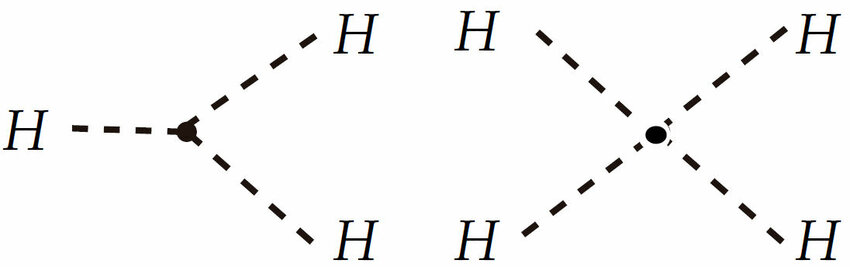
\includegraphics[width= .5\textwidth]{Figures/Introduction/HiggsSelfInt.png}
\caption{Feynman diagrams arising from the presence of the Higgs self-interaction terms in the SM Lagrangian.}
\label{Figure:Introduction_HiggsSelf}
\end{figure}

Remarkably, fermions in the SM also acquire masses via the Higgs mechanism through Yukawa interactions~\cite{YukawaInteractions}. The Yukawa part of the Lagrangian for a generic fermion $f$ can be written as,


\begin{equation}
    \mathcal{L}_{Yukawa}^f = \underbrace{-\frac{g_f}{\sqrt{2}}\nu(\overline{\psi_L}\psi_R + \overline{\psi_R} \psi_L)}_{\text{mass term}} \underbrace{- \frac{g_f}{\sqrt{2}}h(\overline{\psi_L}\psi_R + \overline{\psi_R} \psi_L)}_{\text{interaction term}}
\end{equation}

where $\psi_L$ and $\psi_R$ are the left-handed and right-handed chiral fields, and the first term gives the mass of fermionic mass $m_f = g_f\nu / \sqrt{2}$. The second term in the Lagrangian describes the coupling between the fermion and the Higgs boson itself, interestingly indicating that heavier fermions couple stronger to the Higgs.

\section{The Higgs boson}

Undoubtedly, one of the most significant achievements in modern physics, is the observation of the long-sought fundamental boson, the Higgs. The confirmation of its existence came back in 2012, when the ATLAS and CMS Collaborations~\cite{Higgs_ATLAS,Higgs_CMS} jointly announced its discovery, marking the completion of the SM particle content. Soon after its discovery, both collaborations conducted several measurements exploring the properties of the Higgs, demonstrating that the observed Higgs looks very much alike the SM Higgs~\cite{HiggsParity_1,HiggsParity_2}. One important test lies in the Higgs boson couplings with the most recent measurements of the coupling strengths~\cite{CMS_Couplings_Measurement} being consistent with the SM prediction, as presented in Fig.~\ref{Figure:Introduction_CMScouplings}.

\begin{figure}[h]
\centering
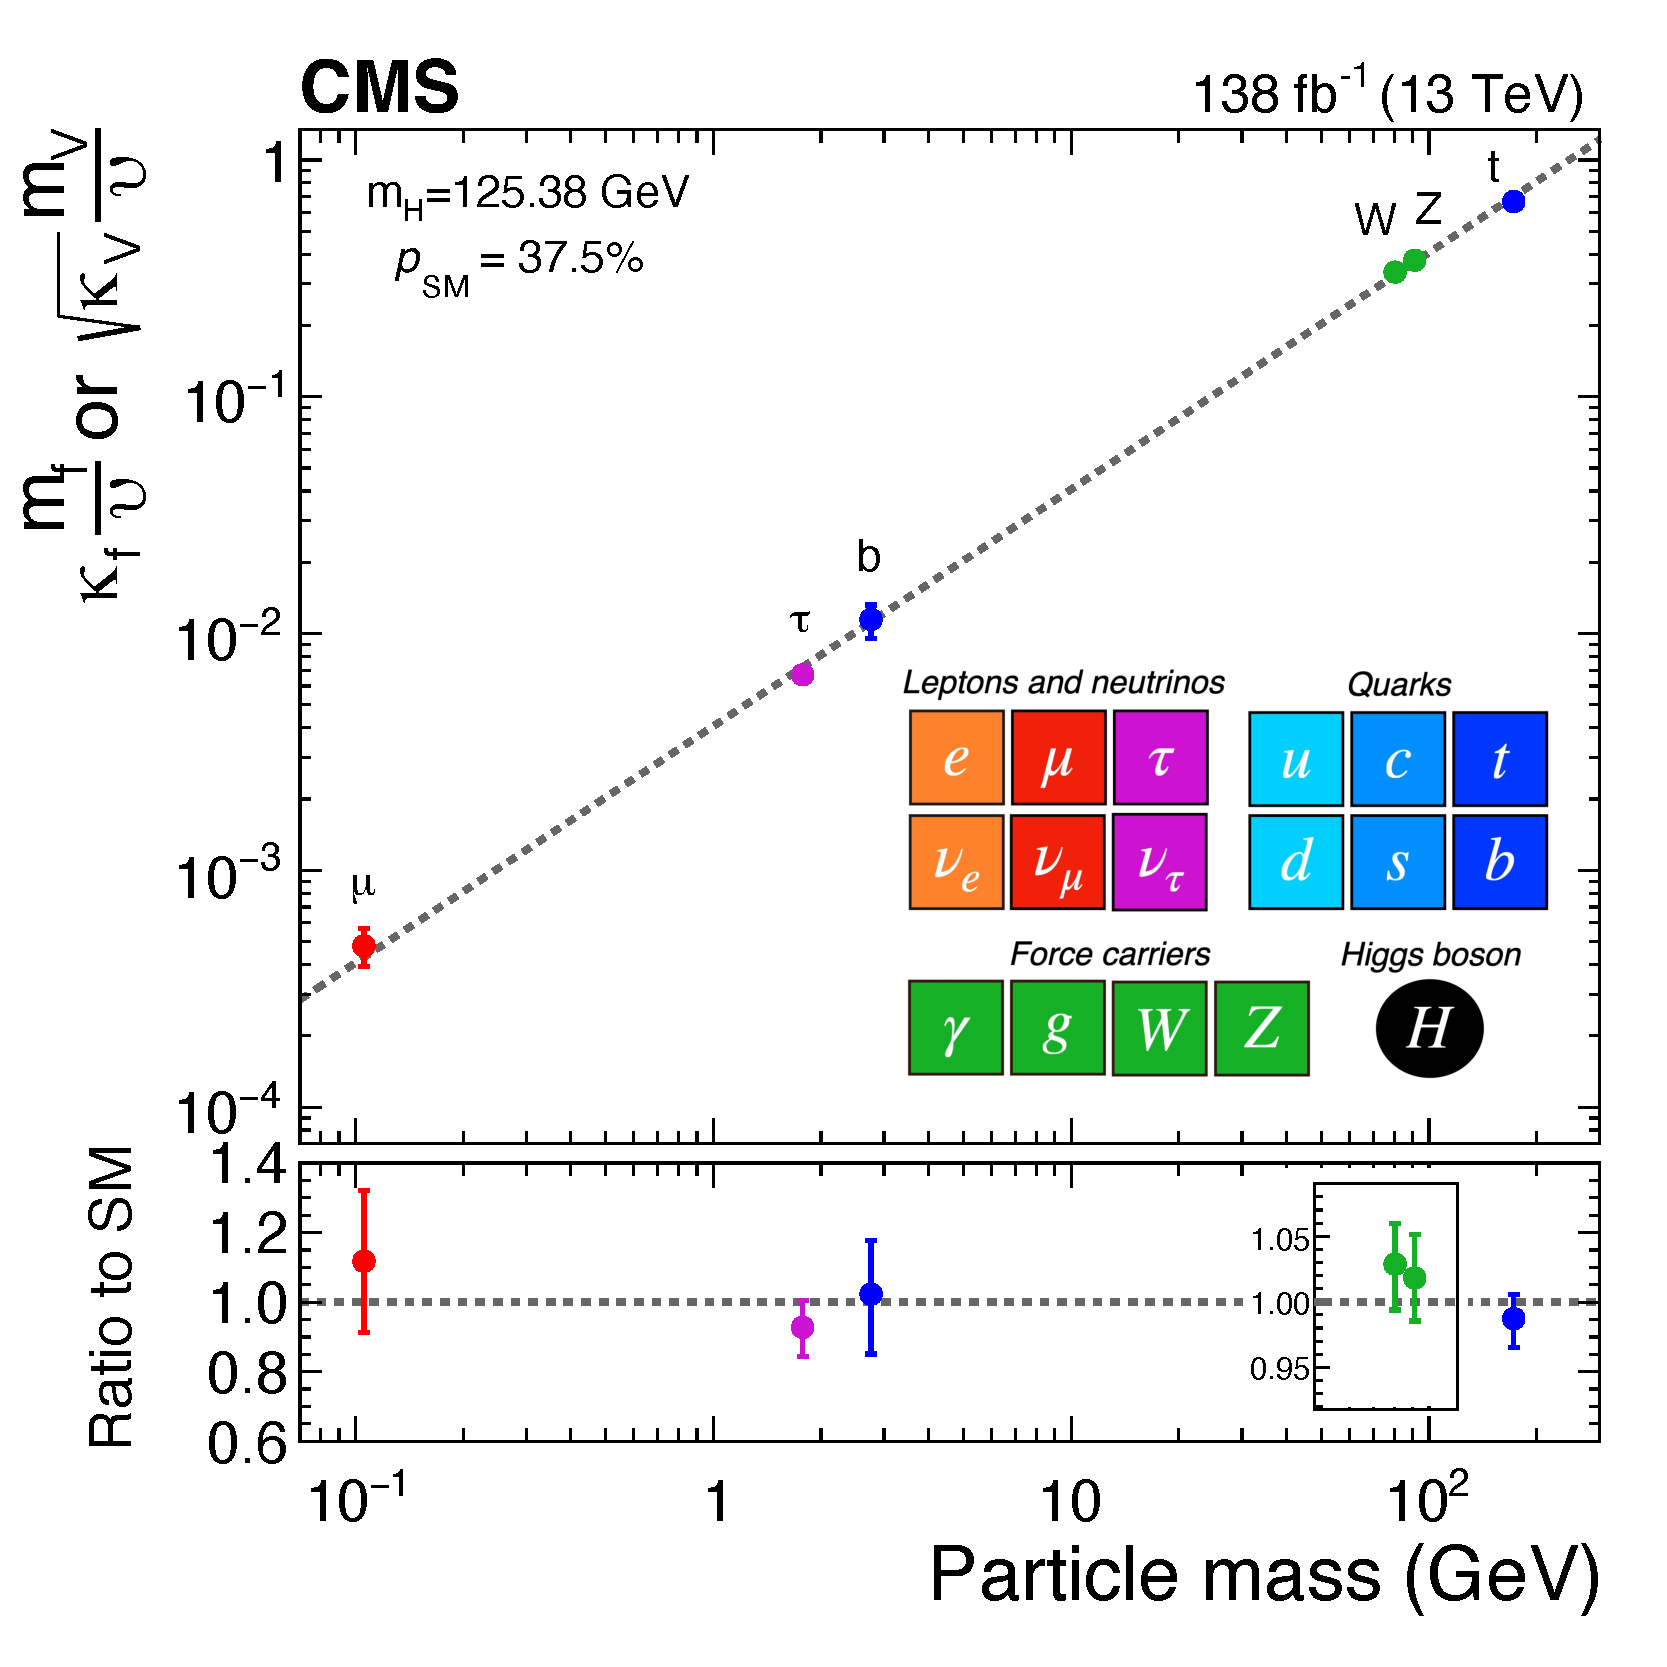
\includegraphics[width= .7\textwidth]{Figures/Introduction/CMS_Higgs_FermionCouplings.pdf}
\caption{The measured coupling strength modifiers of the Higgs boson to fermions and heavy gauge bosons, presented as a function of the fermionic/bosonic masses. For gauge bosons, the "reduced" coupling modifiers are presented, to keep a linear proportionality to the mass~\cite{CMS_Couplings_Measurement}.}
\label{Figure:Introduction_CMScouplings}
\end{figure}

\subsection{Higgs boson production}

At the \ac{LHC}, the Higgs boson is produced via four major production modes; gluon-gluon fusion (ggH), vector boson fusion (VBF), vector boson associated production (VH), and $t\overline{t}$-associated production (ttH); listed in order of decreasing cross-section. In addition to the dominant production modes, the Higgs can still be produced in different ways \eg in association with a single-top (tH). The Feynman diagrams of the dominant modes are displayed in Fig.~\ref{Figure:Introduction_HiggsProductionModes} while their respective cross-sections at $\sqrt{s}$ = 13$\TeV$ and $\sqrt{s}$ = 13.6$\TeV$ are displayed in Table~\ref{Table:Introduction_HiggsProduction_XS}. 

\begin{figure}[h]
\centering
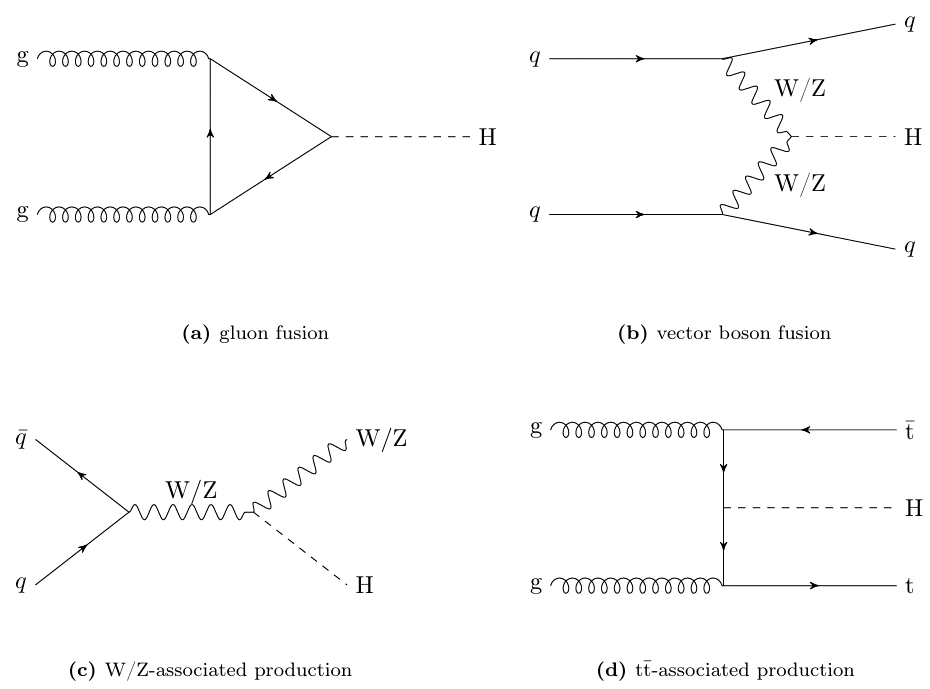
\includegraphics[width= .9\textwidth]{Figures/Introduction/Higgs_ProductionModes.png}
\caption{TODO }
\label{Figure:Introduction_HiggsProductionModes}
\end{figure}

\begin{table}[h]
\centering
\begin{tabular}{l|c|c|c|c|c}
\hline
Production mode                   & ggH   & VBF   & WH    & ZH     & ttH  \\ \hline
Cross section @ 13~$\TeV$ {[}pb{]}   & 48.6  & 3.78  & 1.37  & 0.76   & 0.51 \\
\hline
Cross section @ 13.6~$\TeV$ {[}pb{]} & 52.23 & 4.078 & 1.457 & 0.9439 & 0.57
\end{tabular}
\caption{Cross sections of the dominant Higgs production mechanisms in the SM. Derived for $\text{m}_H = 125\GeV$ and presented for both $\sqrt{\sigma}=13\TeV$ and $\sqrt{\sigma}=13.6\TeV$~\cite{HiggsProduction_XS}}
\label{Table:Introduction_HiggsProduction_XS}
\end{table}

The ggH production mode is clearly the most dominant one proceeding via an internal quark loop, consequence of the Higgs not directly coupling to the gluon. Despite its dominance, other production modes such as VBF have an interesting feature, additional objects in their final states. These distinct topologies can be leveraged to reduce backgrounds. In particular, the VBF production mode is characterised by two additional energetic jets which tend to have a large spatial separation and a high invariant mass.

\subsection{Higgs boson decays}

The Higgs boson is an unstable particle, decaying almost immediately after its production~\cite{HiggsUnstable}, with its inference only possible from the decay products. The dominant SM Higgs decays channels are listed in Table~\ref{Table:Introduction_HiggsBranchingFractions}, clearly showing that $H\rightarrow b\overline{b}$ is the dominant decay mode. 

\begin{table}[h]
\begin{tabular}{l|c|c|c|c|c|c|c|c}
\hline
Decay Mode                  & $b\overline{b}$    & $WW^*$    & gg   & $\tau\tau$   & $c\overline{c}$   & $ZZ^*$      & $\gamma\gamma$ & $\mu\mu$ \\ \hline
Branching Fraction {[}\%{]} & 58.24 & 21.37 & 8.19 & 6.27 & 2.89 & 2.61 & 0.23                            & 0.02
\end{tabular}
\caption{Branching fractions, $\text{B}_f$, of the main SM Higgs boson decay channel for $\text{m}_H = 125\GeV$~\cite{HiggsProduction_XS} where for a particular final state $f$, $\text{B}_f = \Gamma_f/\Gamma_H$}, with $\Gamma_f$ and $\Gamma_H$ being the decay width of the final state and the Higgs boson respectively.

\label{Table:Introduction_HiggsBranchingFractions}
\end{table}

However, the sensitivity of this event is heavily impacted by the presence of large hadronic background. The Higgs discovery was only possible after a combination of several of the decay channels; $H\rightarrow ZZ \rightarrow 4l$, $H\rightarrow \gamma \gamma$, $H\rightarrow WW^*$, $H\rightarrow \tau\tau$ and $H\rightarrow b\overline{b}$, with the di-photon and 4 lepton decay channels being the main contributors. Particularly interesting is the $H\rightarrow \tau\tau$ decay mode, providing a relatively large branching fraction, while being less impaired by backgrounds than $H\rightarrow b\overline{b}$.
